% ==============================================================================
% VLIZ Scientific Research Poster Template - tikzposter
% ==============================================================================
% Matches the official VLIZ institutional brand:
% - Exact top sea-teal banner (#91C8CD) with VLIZ wave logo and vliz.be
% - Left-aligned Subtitle (teal #31B7BC), Title (navy #3057A5), and Authors (#231F20)
% - Hybrid Central Highlight: Full-width hero callout / map section
% - 3-column structured grid below for Context, Methods, and Results
% ==============================================================================

\documentclass[
  25pt,
  a0paper,
  portrait,
  margin=0mm,
  innermargin=15mm,
  blockverticalspace=14mm,
  colspace=14mm,
  subcolspace=8mm
]{tikzposter}

\usepackage{graphicx}
\graphicspath{{assets/}{posters/vliz-poster/assets/}{templates/posters/assets/}{../assets/}}
\usepackage{amsmath,amssymb}
\usepackage{booktabs}
\usepackage{qrcode}
\usepackage{hyperref}
\usepackage{tikz}
\usetikzlibrary{positioning,calc}

% ------------------------------------------------------------------------------
% VLIZ Color Palette
% ------------------------------------------------------------------------------
\definecolor{vlizBanner}{HTML}{91C8CD}       % Exact Sea-teal from template
\definecolor{vlizTeal}{HTML}{31B7BC}         % Vibrant teal subtitle
\definecolor{vlizNavy}{HTML}{3057A5}         % Corporate Navy
\definecolor{vlizCharcoal}{HTML}{231F20}     % Dark Charcoal author font
\definecolor{vlizSlateText}{HTML}{1E293B}    % Main body text
\definecolor{vlizSlateMuted}{HTML}{64748B}   % Muted text
\definecolor{vlizCardBg}{HTML}{FFFFFF}       % White card background
\definecolor{vlizHeroBg}{HTML}{F8FAFC}       % Soft sky/slate hero card background
\definecolor{vlizBorder}{HTML}{CBD5E1}       % Card border

% Set custom tikzposter style
\definecolorstyle{VLIZStyle}{
  \definecolor{colorOne}{HTML}{3057A5}
  \definecolor{colorTwo}{HTML}{31B7BC}
  \definecolor{colorThree}{HTML}{91C8CD}
}{
  % Background Colors
  \colorlet{backgroundcolor}{white}
  \colorlet{framecolor}{white}
  % Title Colors
  \colorlet{titlefgcolor}{vlizNavy}
  \colorlet{titlebgcolor}{white}
  % Block Colors
  \colorlet{blocktitlebgcolor}{white}
  \colorlet{blocktitlefgcolor}{vlizNavy}
  \colorlet{blockbodybgcolor}{vlizCardBg}
  \colorlet{blockbodyfgcolor}{vlizSlateText}
}

\usetheme{Default}
\usecolorstyle{VLIZStyle}

% Custom block style: Clean card with colored title and subtle border
\defineblockstyle{VLIZBlock}{
  titlewidthscale=1.0, bodywidthscale=1.0,
  titleoffsetx=0pt, titleoffsety=0pt, bodyoffsetx=0pt, bodyoffsety=0pt,
  bodyverticalshift=0pt, roundedcorners=15, linewidth=2pt,
  titleinnersep=8mm, bodyinnersep=10mm
}{
  \draw[color=vlizBorder, fill=blockbodybgcolor, rounded corners=15, line width=2pt]
    (blockbody.south west) rectangle (blocktitle.north east);
}
\useblockstyle{VLIZBlock}

% Suppress default centered title
\title{}
\author{}
\institute{}

\begin{document}

% ==============================================================================
% 1. TOP BANNER (Exact VLIZ Vector Header)
% ==============================================================================
% 1a. Native Sea-Teal Banner Background Fill
\fill[vlizBanner] (-0.5\paperwidth, 0.5\paperheight)
  rectangle (0.5\paperwidth, {0.5\paperheight - 0.119\paperheight});

% 1b. Vector VLIZ Logo (Traced SVG: Crisp White Wave + VLIZ Navy Typography)
\node[anchor=west, inner sep=0pt] at ({-0.5\paperwidth + 0.088\paperwidth}, {0.5\paperheight - 0.0595\paperheight}) {
  \includegraphics[height=0.068\paperheight]{vliz_logo.pdf}
};

% 1c. Sharp Native Vector Typography for URL
\node[anchor=east, inner sep=0pt] at ({0.5\paperwidth - 0.088\paperwidth}, {0.5\paperheight - 0.0595\paperheight}) {
  {\color{vlizNavy}\sffamily\bfseries\fontsize{36pt}{42pt}\selectfont vliz.be}
};

% ==============================================================================
% 2. TITLE & AUTHORS SECTION (Left-Aligned with 8.8% Margin)
% ==============================================================================
\node[anchor=north west, text width=0.84\paperwidth, align=flush left, inner sep=0pt]
  at ({-0.5\paperwidth + 0.088\paperwidth}, {0.5\paperheight - 0.135\paperheight}) {
  % Subtitle
  {\color{vlizTeal}\bfseries\LARGE SUBTITLE / RESEARCH TOPIC \par}
  \vspace{0.4cm}
  % Main Title
  {\color{vlizNavy}\bfseries\fontsize{52pt}{60pt}\selectfont Title poster here Lorem ipsum dolor sit amet, consectetur veniam. \par}
  \vspace{0.6cm}
  % Authors
  {\color{vlizCharcoal}\bfseries\LARGE Jan Peeters, Peter Jansens, Anne De Smet \par}
  \vspace{0.25cm}
  % Affiliations & Contact
  {\color{vlizSlateMuted}\large Flanders Marine Institute (VLIZ), InnovOcean Campus, Jacobsenstraat 1, 8400 Oostende, Belgium \quad $\vert$ \quad Contact: info@vliz.be \par}
};

% ==============================================================================
% Set starting vertical position for tikzposter blocks
% ==============================================================================
\makeatletter
\setlength{\TP@blocktop}{0.5\textheight - 270mm}
\makeatother

% ==============================================================================
% 3. HYBRID CENTRAL HIGHLIGHT (Full Width Hero Takeaway / Map Section)
% ==============================================================================
\block{}{
  \begin{minipage}{0.62\linewidth}
    {\color{vlizNavy}\bfseries\Large CENTRAL HIGHLIGHT \& KEY FINDING \par}
    \vspace{0.3cm}
    \textbf{Core Scientific Discovery:}
    \begin{itemize}
      \item \textbf{Spatial Species Turnover:} Multi-year acoustic telemetry and benthic surveys reveal significant community shifts in the Belgian Part of the North Sea (BPNS).
      \item \textbf{Environmental Forcing:} Salinity gradients, turbidity plumes, and sediment grain size account for 68\% of observed variance ($p < 0.001$).
      \item \textbf{Conservation Baseline:} Establishes empirical thresholds for ecosystem-based marine spatial planning and Marine Protected Area (MPA) management.
    \end{itemize}
  \end{minipage}%
  \hfill
  \begin{minipage}{0.34\linewidth}
    \centering
    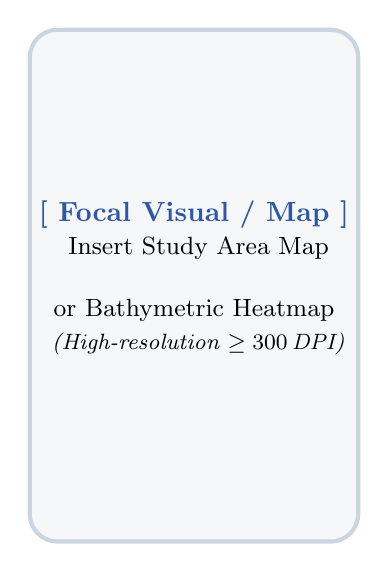
\begin{tikzpicture}
      \node[draw=vlizBorder, fill=vlizBorder!20, rounded corners=10, line width=1.5pt, minimum width=0.33\linewidth, minimum height=6.5cm, align=center] {
        \textbf{\color{vlizNavy} [ Focal Visual / Map ]}\\
        \vspace{0.3cm}
        {\small Insert Study Area Map}\\
        {\small or Bathymetric Heatmap}\\
        \vspace{0.2cm}
        {\footnotesize \textit{(High-resolution $\ge 300$\,DPI)}}
      };
    \end{tikzpicture}
  \end{minipage}
}

% ==============================================================================
% 4. SUPPORTING 3-COLUMN GRID (Context, Methods, Results)
% ==============================================================================
\begin{columns}
  % ---- Column 1: Context & Objectives ----
  \column{0.333}
  
  \block{1. Introduction \& Background}{
    Coastal marine ecosystems face compounding pressures from climate change, offshore infrastructure, and aggregate extraction.
    
    \vspace{0.4cm}
    \textbf{Research Questions:}
    \begin{itemize}
      \item How do benthic functional guilds respond to artificial hard substrate introductions?
      \item Can high-frequency sensor buoys detect early-warning signals for oxygen depletion?
    \end{itemize}
    
    \vspace{0.3cm}
    \textbf{Study Area:} 12 permanent monitoring stations in the Southern Bight of the North Sea.
  }
  
  \block{2. Research Objectives}{
    \begin{enumerate}
      \item Quantify benthic-pelagic coupling dynamics over a 5-year observation cycle.
      \item Validate autonomous biodiversity assessment using environmental DNA (eDNA).
      \item Integrate occurrences into the European Marine Observation Network (EMODnet).
    \end{enumerate}
  }

  % ---- Column 2: Methods & Pipeline ----
  \column{0.334}
  
  \block{3. Methodology \& Instrumentation}{
    \textbf{Multi-Sensor Observational Pipeline:}
    \begin{itemize}
      \item \textbf{Research Cruises:} RV \textit{Simon Stevin} quarterly sampling cruises conducting rosette CTD casts.
      \item \textbf{Acoustic Telemetry:} Permanent acoustic receiver grid recording acoustically tagged fish migrations.
      \item \textbf{Metabarcoding:} High-throughput eDNA sequencing (12S and COI loci) yielding 142 distinct marine taxa.
    \end{itemize}
    
    \vspace{0.3cm}
    \begin{center}
      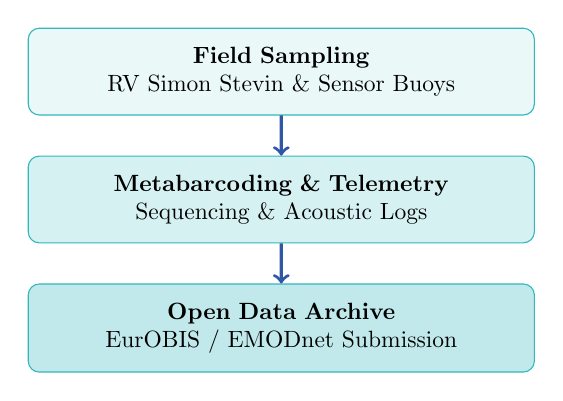
\begin{tikzpicture}[scale=0.85, every node/.style={transform shape}]
        \node[draw=vlizTeal, fill=vlizTeal!10, rounded corners, inner sep=8pt, text width=7cm, align=center] (s1) {\textbf{Field Sampling}\\RV Simon Stevin \& Sensor Buoys};
        \node[draw=vlizTeal, fill=vlizTeal!20, rounded corners, inner sep=8pt, text width=7cm, align=center, below=0.6cm of s1] (s2) {\textbf{Metabarcoding \& Telemetry}\\Sequencing \& Acoustic Logs};
        \node[draw=vlizTeal, fill=vlizTeal!30, rounded corners, inner sep=8pt, text width=7cm, align=center, below=0.6cm of s2] (s3) {\textbf{Open Data Archive}\\EurOBIS / EMODnet Submission};
        \draw[->, very thick, vlizNavy] (s1) -- (s2);
        \draw[->, very thick, vlizNavy] (s2) -- (s3);
      \end{tikzpicture}
    \end{center}
  }
  
  \block{4. Data Quality Standards}{
    All occurrences follow Darwin Core Archive (DwC-A) standards and are curated in the Marine Data Archive (MDA).
  }

  % ---- Column 3: Results & Synthesis ----
  \column{0.333}
  
  \block{5. Results \& Discussion}{
    \textbf{Key Observations:}
    \begin{itemize}
      \item \textbf{Biodiversity Enhancement:} 24\% increase in demersal fish diversity adjacent to artificial reef foundations.
      \item \textbf{Phenology Shift:} Spring phytoplankton bloom advanced by 11 days across the observation period.
      \item \textbf{Turbidity Impact:} High SPM concentrations reduced photic depth by 35\% during storm seasons.
    \end{itemize}
  }
  
  \block{6. Conclusions \& Impact}{
    Long-term automated observatories demonstrate high sensitivity to regional climate variations, providing actionable guidance for maritime spatial planners.
  }

  \block{Scan for Open Data}{
    \begin{center}
      \qrcode[height=4.2cm]{https://www.vliz.be}\\
      \vspace{0.3cm}
      \small \texttt{www.vliz.be/en/marine-data-archive}
    \end{center}
  }
\end{columns}

% ==============================================================================
% 5. FOOTER (Full Width)
% ==============================================================================
\block{}{
  \footnotesize
  \begin{minipage}{0.75\textwidth}
    \textbf{References:} [1] Peeters et al. (2025). \textit{North Sea Observation Network}. J. Mar. Sci. \quad [2] Jansens \& De Smet (2024). \textit{Coastal Baselines}. Oceanol.\\
    \textbf{Acknowledgments:} Supported by the Flanders Marine Institute (VLIZ) and European Horizon Research Infrastructure Grant.
  \end{minipage}%
  \hfill
  \begin{minipage}{0.22\textwidth}
    \raggedleft
    VLIZ Marine Science Day 2026\\
    InnovOcean Campus, Oostende
  \end{minipage}
}

\end{document}
